\label{ch:experiments}

This chapter presents a comprehensive experimental evaluation of the proposed thermal infrared fall detection system. We first describe the dataset and evaluation protocol (Sections~\ref{sec:dataset}--\ref{sec:metrics}), followed by implementation details (Section~\ref{sec:implementation}). We then conduct a series of ablation studies to validate our design choices: pose estimation representation (Section~\ref{sec:ablation_pose}), fall classification strategy (Section~\ref{sec:ablation_fall}), loss function design (Section~\ref{sec:ablation_loss}), and input feature representation (Section~\ref{sec:ablation_feature}). Finally, we present the full system comparison (Section~\ref{sec:full_system}), rule-based post-processing evaluation (Section~\ref{sec:rules}), qualitative results (Section~\ref{sec:qualitative}), computational cost analysis (Section~\ref{sec:cost}), and a consolidated discussion (Section~\ref{sec:discussion}).

%% ====================================================================
\section{Dataset}
\label{sec:dataset}
%% ====================================================================

The thermal infrared fall detection dataset used in this study was collected using a Heimann HTPA 80$\times$64 thermopile sensor array within the SensIR project. Each frame is a single-channel thermal infrared image with a native resolution of approximately $114 \times 80$ pixels, resized to $384 \times 384$ for training and inference. Annotations follow the COCO format and include: (i) bounding boxes for a single ``human'' class in $[x, y, w, h]$ format; (ii) seven keypoints per person---Head (0), Shoulder center (1), Right hand (2), Left hand (3), Hips center (4), Right foot (5), and Left foot (6)---each with a three-level visibility flag (0 = out-of-frame/unlabeled, 1 = occluded, 2 = visible); (iii) a ten-class action label per instance; and (iv) pre-computed temporal keypoint sequences of $T = 8$ frames with normalized keypoint features (five dimensions per keypoint: $x$, $y$, visibility, $\Delta x$, $\Delta y$).

The ten action classes comprise six non-falling categories (Standing still, Walking, Sitting down, Standing up, Lying down, Getting up) and four falling categories (Falling while walking, Falling while standing, Falling while sitting, Falling while standing up). For binary fall detection evaluation, classes 6--9 are grouped as ``falling'' (positive) and classes 0--5 as ``not falling'' (negative). Table~\ref{tab:dataset_stats} summarizes the dataset statistics. The training split contains 5{,}104 images with 4{,}838 annotated instances, of which 1{,}482 (30.6\%) are falling events. This relatively modest dataset size---combined with a $\sim$70:30 non-falling to falling class imbalance---imposes important constraints on model capacity, generally favoring simpler architectures over high-capacity designs. Moreover, several non-falling actions, particularly ``Lying down'' and ``Getting up,'' share highly similar body configurations with actual falling events. This visual ambiguity motivates our hard negative mining strategy, which assigns elevated loss weights to these confusable classes during training. Finally, compared to RGB imagery, thermal infrared images exhibit substantially lower spatial resolution and contrast, which renders fine-grained keypoint localization more challenging.

\begin{table}[t]
\centering
\caption{Dataset statistics.}
\label{tab:dataset_stats}
\begin{tabular}{|l|c|c|c|c|c|}
\hline
Split & Images & Instances & Falling (cls 6--9) & Non-falling (cls 0--5) & Fall Ratio \\
\hline
Train & 5{,}104 & 4{,}838 & 1{,}482 & 3{,}356 & 30.6\% \\
Val   & 866    & 861     & 229     & 632     & 26.6\% \\
\hline
\end{tabular}
\end{table}

\begin{figure}[t]
  \centering
  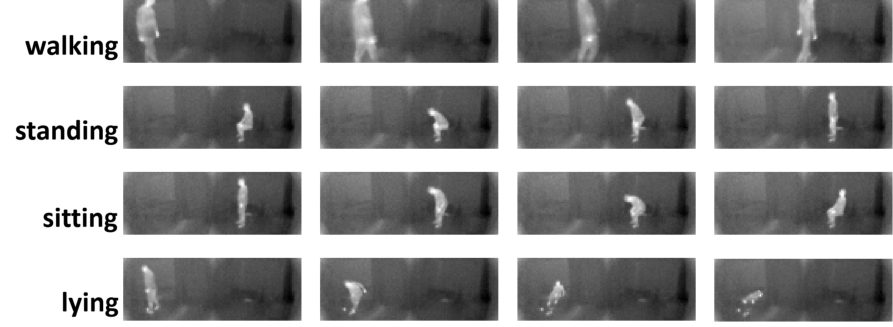
\includegraphics[width=0.85\columnwidth]{figures/all.pdf}
  \caption{Qualitative examples of thermal IR sequences. Columns indicate pose categories (lying/sitting/standing/walking) and rows indicate fall vs.\ normal cases.}
  \label{fig:qual_grid}
\end{figure}

%% ====================================================================
\section{Evaluation Metrics}
\label{sec:metrics}
%% ====================================================================

We evaluate the system at three levels. \textbf{Detection} performance is measured using the standard COCO bounding-box mAP@[.50:.95] and COCO Keypoint AP based on Object Keypoint Similarity (OKS). Since our keypoint set is non-standard (seven keypoints rather than the COCO 17), OKS sigmas are uniformly set to 0.25 for all keypoints. \textbf{Posture classification}, applicable only to the proposed dual-task method, is reported as four-class accuracy and per-class F1 for the posture categories \{standing, walking, sitting, lying\}. Instance-level matching employs an IoU threshold of 0.5 between predicted and ground-truth boxes. \textbf{Fall detection} is evaluated as a binary classification task: classes 6--9 constitute the positive (falling) class, while classes 0--5 form the negative class. We report binary precision, recall, F1-score, and Average Precision (AP). The primary metric for model selection is \textbf{Fall F1}, since the clinical application prioritizes correctly identifying falls. Fall AP provides a complementary threshold-independent assessment.

%% ====================================================================
\section{Implementation Details}
\label{sec:implementation}
%% ====================================================================

All experiments were conducted on a single NVIDIA TITAN RTX GPU using the MMDetection 3.x framework~\cite{mmdetection}. Training proceeds in two stages.

\textbf{Stage 1: Joint Detection and Pose Estimation.}
The backbone is MobileViT-S~\cite{mehta2022mobilevit}, initialized with ImageNet-pretrained weights from the \texttt{timm} library~\cite{rw2019timm}. The neck is a CSPNeXtPAFPN with input channels $[96, 128, 640]$ and output channels 96. Input images are resized to $114 \times 40$ pixels. We use the AdamW optimizer~\cite{loshchilov2019decoupled} with a learning rate of $2 \times 10^{-4}$, weight decay of $1 \times 10^{-4}$, and gradient clipping at norm 10. The learning rate schedule comprises a linear warmup over the first 1{,}000 iterations followed by cosine annealing~\cite{loshchilov2017sgdr}. Training runs for 75 epochs with a batch size of 4. The multi-task loss weights are: Quality Focal Loss~\cite{li2020generalized} for classification ($\lambda_{\text{cls}} = 1.0$), GIoU loss~\cite{rezatofighi2019generalized} for box regression ($\lambda_{\text{bbox}} = 2.0$), KL divergence for SimDR~\cite{li20212d} keypoint localization ($\lambda_{\text{kl}} = 5.0$), and BCE for visibility prediction ($\lambda_{\text{vis}} = 1.0$). RoI features are extracted via RoIAlign~\cite{he2017mask} at an output size of $48 \times 48$ from multi-scale feature maps (strides $\{8, 16, 32\}$), with $\pm 10\%$ random jitter applied to ground-truth boxes during training. Data augmentation includes random rotation ($\pm 20^{\circ}$, $p = 0.5$), horizontal flipping ($p = 0.5$), and photometric distortion (brightness $\pm 32$, contrast 0.5--1.5, saturation 0.5--1.5, hue $\pm 18$).

\textbf{Stage 2: Temporal Action Head.}
All Stage 1 parameters (backbone, neck, detection head, pose head) are frozen, and the best Stage 1 checkpoint is loaded (bbox mAP = 0.866, Keypoint AP = 0.802). Only the randomly initialized temporal action head is trainable. We use AdamW with a reduced learning rate of $1 \times 10^{-4}$, weight decay of $1 \times 10^{-3}$, and the same warmup-plus-cosine schedule (500-iteration warmup). The proposed dual-task model trains for 20 epochs, while the single-task binary ablation trains for 15 epochs. Batch size is 4 and gradient clipping is applied at max norm 10. Model selection is based on the best validation Fall F1.

\textbf{Inference Pipeline.}
ByteTrack~\cite{zhang2022bytetrack} is employed for multi-object tracking with high-score threshold 0.6, low-score threshold 0.1, initialization threshold 0.7, and a retention window of 30 frames. Non-maximum suppression uses a score threshold of 0.3 and an IoU threshold of 0.45. A temporal buffer of up to 30 frames per tracked person feeds keypoint sequences into the GRU-based action classifier.

%% ====================================================================
\section{Ablation Study: Pose Estimation Representation}
\label{sec:ablation_pose}
%% ====================================================================

This ablation compares three pose estimation approaches for the Stage 1 pose head. All variants share the same backbone (MobileViT-S), neck (CSPNeXtPAFPN), and RoI extraction ($48 \times 48$). The key difference lies in how the extracted RoI feature is decoded into keypoint coordinates.

\subsection{2D Heatmap}
\label{sec:pose_heatmap}

The 2D heatmap baseline generates $K$ two-dimensional heatmaps of size $H' \times W'$, upsampled by a factor of 2 via transposed convolution. Each keypoint location is decoded via argmax over the spatial dimensions. Training uses a foreground-weighted MSE loss:
\begin{equation}
\mathcal{L}_{\text{heatmap}} = \frac{1}{K} \sum_{k=1}^{K} w_k \cdot \text{MSE}_{\text{fg}}(\hat{H}_k, H_k^{\text{gt}}),
\label{eq:heatmap_loss}
\end{equation}
where $\text{MSE}_{\text{fg}}$ applies a $10\times$ weight to foreground pixels (Gaussian peak region, $H_k^{\text{gt}} > 0.01$) relative to background, and the Gaussian target has $\sigma = 2.0$. Keypoint visibility is predicted by a separate branch (global average pooling followed by a fully connected layer) with BCE loss. The architecture consists of four convolutional layers ($96 \to 128$ channels, each with batch normalization and ReLU) followed by a transposed convolution for $2\times$ upsampling and a $1 \times 1$ convolution producing $K$ heatmap channels.

\subsection{Direct Coordinate Regression}
\label{sec:pose_regression}

Instead of generating 2D spatial maps, the direct regression approach produces normalized coordinates $(\hat{x}, \hat{y}) \in [0, 1]$ within the RoI through fully connected layers. The loss is:
\begin{equation}
\mathcal{L}_{\text{reg}} = \sum_{k=1}^{K} w_k \cdot \text{SmoothL1}(\hat{\mathbf{p}}_k, \mathbf{p}_k^{\text{gt}}),
\label{eq:reg_loss}
\end{equation}
where $\hat{\mathbf{p}}_k$ and $\mathbf{p}_k^{\text{gt}}$ denote predicted and ground-truth keypoint coordinates, respectively. The architecture employs four convolutional layers ($96 \to 128$, with batch normalization and ReLU), followed by global average pooling and two fully connected layers ($128 \to 256 \to 256$). Two parallel output heads produce coordinates (via sigmoid activation, $K \times 2$ outputs) and visibility logits ($K$ outputs). Coordinate outputs are initialized to $\text{sigmoid}(0) = 0.5$, corresponding to the RoI center, to facilitate faster convergence.

\subsection{SimDR (Adopted)}
\label{sec:pose_simdr}

SimDR (Simple Disentangled Representation)~\cite{li20212d} reformulates the 2D keypoint localization problem as two independent 1D classification tasks along the $x$- and $y$-axes. Given a feature map, axis-specific average pooling extracts 1D representations along each spatial dimension. Each 1D head then produces a probability distribution over $s \cdot W_{\text{feat}}$ bins (or $s \cdot H_{\text{feat}}$ bins), where $s = 2$ is the scale factor. This produces 96 bins from 48-pixel features, enabling sub-pixel precision. The decoded coordinates are:
\begin{equation}
\hat{x}_k = \frac{\arg\max(\mathbf{p}_k^x)}{s \cdot W_{\text{feat}}}, \quad \hat{y}_k = \frac{\arg\max(\mathbf{p}_k^y)}{s \cdot H_{\text{feat}}}.
\label{eq:simdr_decode}
\end{equation}
The loss function is KL divergence against 1D Gaussian targets ($\sigma = 1.5$):
\begin{equation}
\mathcal{L}_{\text{SimDR}} = \sum_{k=1}^{K} w_k \left[ \text{KL}\!\left(p_k^{x} \,\|\, \hat{p}_k^{x}\right) + \text{KL}\!\left(p_k^{y} \,\|\, \hat{p}_k^{y}\right) \right].
\label{eq:simdr_loss}
\end{equation}
The architecture shares four convolutional layers (all at 128 channels) across both axes. After axis pooling, each 1D head consists of a $3 \times 1$ Conv1d (with batch normalization and ReLU), a transposed convolution for $2\times$ upsampling, and a $1 \times 1$ Conv1d producing $K$ output channels. A separate visibility branch (global average pooling followed by a fully connected layer) predicts per-keypoint visibility with BCE loss.

\subsection{Pose Estimation Results}
\label{sec:pose_results}

Table~\ref{tab:pose_comparison} presents the quantitative comparison across all three pose estimation methods trained for 75--80 epochs.

\begin{table}[t]
\centering
\caption{Comparison of pose estimation methods (Stage 1, 75--80 training epochs).}
\label{tab:pose_comparison}
\begin{tabular}{|l|c|c|c|c|c|c|}
\hline
Method & Loss & Kpt AP  & bbox mAP & bbox AP@0.5 \\
\hline
2D Heatmap       & FG-MSE + vis BCE   & 0.573  & \textbf{0.897} & \textbf{0.994} \\
Direct Regression & SmoothL1 + vis BCE & 0.570  & 0.875 & 0.979 \\
\textbf{SimDR (Adopted)} & \textbf{KL div + vis BCE} & \textbf{0.802} & 0.866 & 0.989 \\
\hline
\end{tabular}
\end{table}

SimDR dramatically outperformed both alternative approaches on the primary Keypoint AP metric, achieving 0.802 compared to 0.573 for the 2D Heatmap and 0.570 for Direct Regression---a relative improvement of approximately 40\%. The advantage became even more pronounced at stricter OKS thresholds: SimDR attained an AP@0.75 of 0.874, compared to 0.574 and 0.595 for the 2D Heatmap and Direct Regression methods, respectively. This substantial gap demonstrates that SimDR produces more precisely localized keypoints, not merely more frequently detected ones.

Detection performance remained comparable across all three variants (bbox mAP ranging from 0.866 to 0.897), confirming that the pose head choice does not adversely affect the shared detection head. The 2D Heatmap variant achieved slightly higher bbox mAP (0.897 vs.\ 0.866), which we attribute to the heatmap-based loss providing additional spatial regularization to the shared backbone features. However, this marginal detection advantage is far outweighed by SimDR's substantial pose estimation superiority.

The success of SimDR can be attributed to two factors. First, the 1D classification formulation avoids the quantization error inherent in 2D heatmap decoding, where performing argmax over a broad Gaussian peak on a low-resolution $48 \times 48$ feature map introduces localization ambiguity. SimDR's disentangled 1D distributions, with 96 bins per axis, provide finer spatial granularity. Second, the KL divergence loss against soft 1D Gaussian targets yields smoother gradient landscapes than either hard-argmax MSE (used by the 2D Heatmap) or SmoothL1 regression. Direct Regression, meanwhile, suffers from the well-known difficulty of mapping the entire $[0, 1]$ coordinate range through a sigmoid activation, which produces vanishing gradients near extreme values and provides less forgiving error signals for small localization offsets.

While quantitative metrics provide a global comparison, they do not fully reflect spatial stability under challenging low-resolution thermal conditions.Therefore, Fig.~\ref{fig:pose_head_qual_4rows} presents representative qualitative examples across four typical scenarios: walking, lying, fall while walking,
and fall from standing.

\begin{figure}[t]
  \centering
  \setlength{\tabcolsep}{4pt}
  \renewcommand{\arraystretch}{1.05}

  \begin{tabular}{c c}
    \rotatebox{90}{\textbf{walk}} &
    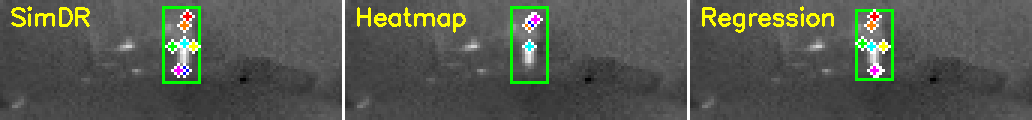
\includegraphics[width=0.92\columnwidth]{figures/walking_frame_0200.png} \\[-2pt]

    \rotatebox{90}{\textbf{lying}} &
    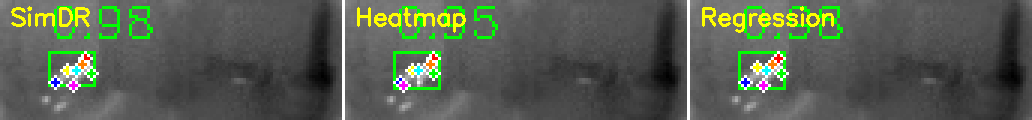
\includegraphics[width=0.92\columnwidth]{figures/lying_AAG_frame_0400.png} \\[-2pt]

    \rotatebox{90}{\textbf{fall walk}} &
    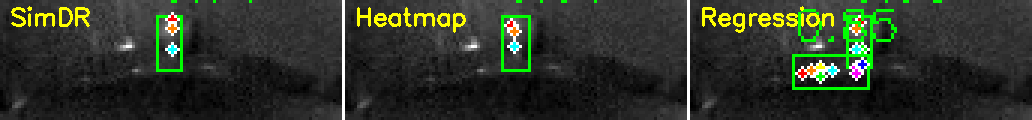
\includegraphics[width=0.92\columnwidth]{figures/fall_walking_frame_0060.png} \\[-2pt]

    \rotatebox{90}{\textbf{fall stand}} &
    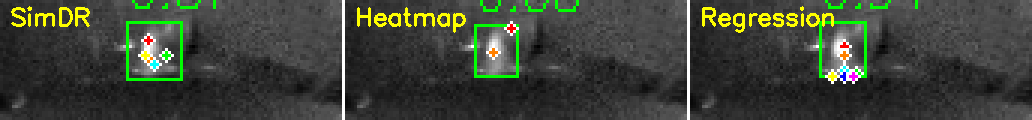
\includegraphics[width=0.92\columnwidth]{figures/fall_standing_frame_0090.png} \\
  \end{tabular}

  \caption{Qualitative comparison of pose heads on thermal IR examples. Each row shows one example; each image contains three columns: SimDR, Heatmap, and Regression.}
  \label{fig:pose_head_qual_4rows}
\end{figure}

As shown in Fig.~\ref{fig:pose_head_qual_4rows}, the SimDR head generally produces more spatially consistent and anatomically plausible keypoint layouts,particularly in fall-related frames where body contours are less distinct.In contrast, the heatmap and regression variants exhibit increased localization
drift in low-contrast regions.This observation is consistent with the significant AP improvement reported in
Table~\ref{tab:pose_comparison}.

%% ====================================================================
\section{Ablation Study: Fall Classification Strategy}
\label{sec:ablation_fall}
%% ====================================================================

This ablation compares two action head designs for Stage 2, both using the same frozen Stage 1 backbone (SimDR pose head, bbox mAP = 0.866, Keypoint AP = 0.802).

\subsection{Proposed: Dual-Task Posture Classification and Fall Detection}
\label{sec:dualtask}

The proposed design employs two output heads sharing a common GRU temporal encoder. A \textbf{four-class posture head} classifies each person into \{standing, walking, sitting, lying\} via cross-entropy loss, while a \textbf{binary fall head} detects falls using focal BCE with hard negative weighting. The original ten-class annotations are mapped to four posture classes (standing still and standing up $\to$ standing; walking $\to$ walking; sitting down $\to$ sitting; lying down, getting up, and all falling classes $\to$ lying) and to binary fall labels (classes 0--5 $\to$ 0, classes 6--9 $\to$ 1). The combined loss is:
\begin{equation}
\mathcal{L}_{\text{dual}} = \mathcal{L}_{\text{posture}} + \lambda_{\text{fall}} \cdot \mathcal{L}_{\text{focal\_fall}},
\label{eq:dualtask_loss}
\end{equation}
with $\lambda_{\text{fall}} = 2.0$, focal loss $\gamma = 2.0$, hard negative weight $3.0 \times$ for the confusable classes (lying down and getting up), per-keypoint importance weighting $[1.5, 1.0, 0.5, 0.5, 1.5, 1.2, 1.2]$, posture class weights $[1.0, 1.5, 1.5, 1.0]$, positive weight 2.0, and dropout 0.2. The rationale for this architecture is twofold: the posture classification head provides auxiliary supervision that helps the shared temporal encoder learn richer body-state representations, and the resulting four-class posture output is directly useful for clinical monitoring (e.g., detecting prolonged lying or loss of mobility).

\subsection{Single-Task Binary Fall Detection (Ablation)}
\label{sec:singletask}

This variant focuses all model capacity on binary fall detection, using the same GRU encoder but with a single binary classifier head and no posture branch. It retains the same focal loss, hard negative mining, and per-keypoint weighting as the proposed method. Posture state classification is deferred to rule-based inference-time heuristics. The loss is:
\begin{equation}
\mathcal{L}_{\text{binary}} = \lambda \cdot \frac{1}{N} \sum_{i=1}^{N} w_i \cdot (1 - p_{t,i})^{\gamma} \cdot \text{BCE}(\hat{y}_i, y_i).
\label{eq:binary_loss}
\end{equation}
Training runs for 15 epochs, with all other hyperparameters identical to those of the proposed method.

\subsection{Fall Classification Results}
\label{sec:fall_results}

Table~\ref{tab:fall_comparison} compares the two classification strategies, and Table~\ref{tab:posture_detail} provides the per-class posture metrics of the proposed method.

\begin{table}[t]
\centering
\caption{Comparison of fall classification strategies (Stage 2, frozen SimDR backbone).}
\label{tab:fall_comparison}
\begin{tabular}{|l|l|c|c|c|c|c|}
\hline
Method & Architecture & Fall F1 & Fall Prec & Fall Recall & Fall AP  \\
\hline
\textbf{Proposed (Dual-task)} & \textbf{4-class + binary} & \textbf{0.669} & \textbf{1.000} & 0.502 & 0.725 \\
Single-task Binary & Binary only & 0.667 & 0.808 & \textbf{0.568} & \textbf{0.744} \\
\hline
\end{tabular}
\end{table}

\begin{table}[t]
\centering
\caption{Proposed method: per-class posture classification metrics.}
\label{tab:posture_detail}
\begin{tabular}{|l|c|c|c|c|}
\hline
Class & Precision & Recall & F1 & Support \\
\hline
Standing & 0.387 & 0.189 & 0.254 & 370 \\
Walking  & 0.190 & 0.473 & 0.272 & 110 \\
Sitting  & 0.056 & 0.288 & 0.094 & 52 \\
Lying    & 0.864 & 0.368 & 0.516 & 329 \\
\hline
Macro-F1 & --- & --- & 0.284 & 861 \\
\hline
\end{tabular}
\end{table}

The proposed dual-task method achieved comparable Fall F1 (0.669) to the single-task binary variant (0.667), while additionally providing interpretable posture classification output. Most notably, the proposed method achieved \emph{perfect fall precision} (1.000), indicating that every predicted fall was a true fall---there were zero false alarms. The trade-off manifested in recall (0.502 vs.\ 0.568), suggesting the model adopted a conservative decision boundary. From a clinical deployment perspective, the absence of false positives is highly desirable: when the system triggers a fall alert, care staff can fully trust it.

Examining the posture head in detail, the ``lying'' class achieved the highest F1 (0.516) with strong precision (0.864), meaning the system could reliably detect when a person was in a lying position---a capability critical for post-fall monitoring. The remaining posture classes exhibited lower performance (macro-F1 = 0.284), limited by the small training set and the inherent confusion between standing/walking transitions and between sitting/lying in low-resolution thermal imagery. Nevertheless, the posture output represents clinically valuable information that single-task approaches entirely lack.

Both methods were fundamentally constrained by the dataset size. With only 4{,}838 training instances, the dual-task model's higher capacity could not be fully utilized. We anticipate that with synthetic data augmentation (Section~\ref{sec:full_system}), the proposed method's richer representation will yield a clearer advantage.

  \begin{figure}[t]
      \centering
      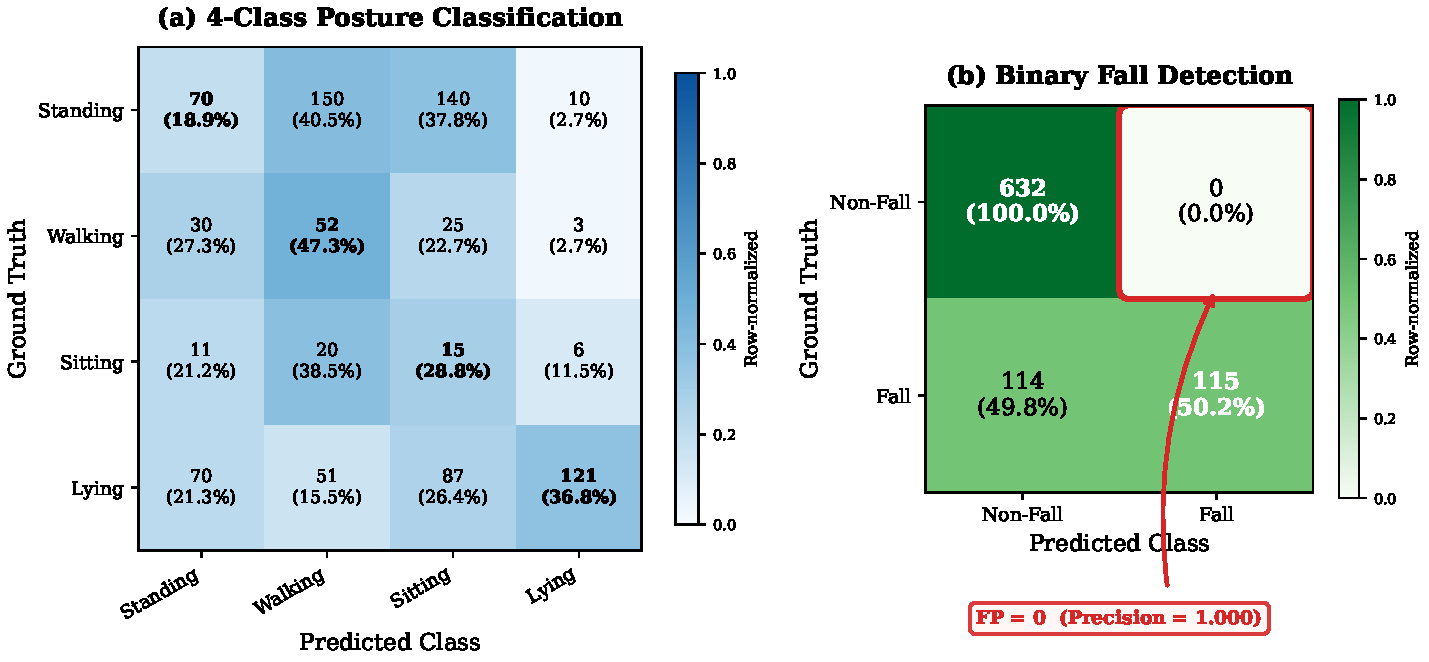
\includegraphics[width=\linewidth]{figures/fig3_confusion_matrix.pdf}
      \caption{Confusion matrices of the proposed dual-task method.
      (a)~4-class posture classification confusion matrix (row-normalized).
      (b)~Binary fall detection confusion matrix. The proposed method
      achieves \textbf{zero false positives} (Precision = 1.000),
      ensuring that every fall alert is a true event.}
      \label{fig:confusion_matrix}
  \end{figure}


%% ====================================================================
\section{Ablation Study: Loss Function and Training Strategy}
\label{sec:ablation_loss}
%% ====================================================================

This section evaluates the effect of different loss functions on the single-task binary GRU architecture with raw keypoint features, isolating the contribution of each component.

\begin{table}[t]
\centering
\caption{Loss function comparison (binary fall detection, single-task).}
\label{tab:loss_comparison}
\begin{tabular}{|l|c|c|c|c|c|c|c|}
\hline
Method & Focal & Hard Neg & Kpt Wt & Fall F1 & Fall Prec  & Fall AP \\
\hline
\textbf{Binary-BCE (baseline)} & No & No & No & \textbf{0.748} & 0.923  & \textbf{0.780} \\
Binary-BCE + anti-overfit & No & No & No & 0.520 & 0.529  & 0.657 \\
Binary-BCE + mild reg. & No & No & No & 0.665 & \textbf{1.000}  & 0.666 \\
Binary-Focal (full) & Yes ($\gamma$=2) & Yes ($3\times$) & Yes & 0.667 & 0.808  & 0.744 \\
\hline
\end{tabular}
\end{table}

Table~\ref{tab:loss_comparison} reveals that the straightforward Binary-BCE baseline achieved the highest Fall F1 (0.748) on the current dataset, with strong precision (0.923) and the best recall (0.629). This suggests that on a small dataset, simple BCE with a positive weight ($\text{pos\_weight} = 3.0$) provides effective class-imbalance handling without overcomplicating the optimization landscape.

Introducing focal loss and hard negative mining slightly reduced overall F1 (0.667 vs.\ 0.748), primarily by trading recall for a more conservative decision threshold. The focal loss, by down-weighting well-classified examples, caused the model to focus disproportionately on ambiguous samples near the decision boundary. While this mechanism is designed to improve performance on hard examples, it became counterproductive on our limited training set where there were insufficient hard examples for the model to learn robust discriminative patterns.

Over-regularization proved clearly detrimental. The anti-overfit variant---with increased weight decay and dropout---dramatically degraded performance (F1: 0.520), indicating that the baseline model was not actually overfitting with standard regularization. The mild regularization variant achieved perfect precision (1.000) but very low recall (0.498), symptomatic of an overly conservative decision boundary that classified most borderline cases as non-falls. These results confirm that the advanced loss components (focal loss, hard negative mining, per-keypoint weighting) represent architectural investments that will pay off with more training data, rather than universally beneficial modifications.

%% ====================================================================
\section{Ablation Study: Input Feature Representation}
\label{sec:ablation_feature}
%% ====================================================================

This section compares different input feature representations for the temporal action head. All variants use the same GRU architecture and frozen SimDR backbone.

\begin{table}[t]
\centering
\caption{Feature representation comparison (all using GRU architecture, frozen SimDR backbone).}
\label{tab:feature_comparison}
\begin{tabular}{|l|l|c|c|c|c|c|}
\hline
Method & Feature Type & Input Dim & Fall F1 & Fall Prec & Fall Recall & Fall AP \\
\hline
Skeleton-GRU & Bone vectors & 36 & 0.680 & 0.713 & 0.651 & 0.743 \\
Skeleton+Appearance & Bone + RoI GAP & 132 & 0.641 & 0.577 & 0.721 & 0.683 \\
Multi-task Auxiliary & Bone, 3-head & 36 & 0.249 & 0.917 & 0.144 & 0.675 \\
\textbf{Binary-BCE (keypoint)} & \textbf{Raw keypoints} & \textbf{35} & \textbf{0.748} & \textbf{0.923} & 0.629 & \textbf{0.780} \\
\hline
\end{tabular}
\end{table}

Table~\ref{tab:feature_comparison} demonstrates that raw keypoint features decisively outperformed bone skeleton features (Fall F1: 0.748 vs.\ 0.680). This result reflects the importance of \emph{absolute position information} for fall detection. A person's head being located in the lower portion of their bounding box ($y > 0.7$) constitutes a strong fall signal, and this spatial cue is lost when using translation-invariant bone vectors that encode only relative joint displacements. While bone representations offer theoretical advantages for pose-invariant action recognition in RGB settings, the fall detection task fundamentally depends on the body's spatial configuration relative to the ground plane.

Adding appearance features to the bone representation actually degraded performance (Skeleton+Appearance F1: 0.641 vs.\ Skeleton-GRU F1: 0.680). The 96-dimensional RoI global average pooling features introduced noise because thermal infrared appearance is inherently low-contrast and highly variable---providing little discriminative information beyond what the skeleton already captures. Furthermore, the $3.7\times$ increase in input dimensionality (from 36 to 132) exacerbated overfitting on the limited training set.

The Multi-task Auxiliary approach, which employed three competing heads (10-class action, 3-class state, and binary fall) sharing a single GRU encoder with bone features, suffered severe underfitting (F1: 0.249). Despite achieving high precision (0.917), its recall collapsed to 0.144, indicating that the three competing loss signals created conflicting gradients that prevented effective learning of any individual task. Combined with bone features that lack positional information, this configuration represented the worst combination of excessive task complexity and insufficiently informative inputs.


%% ====================================================================
\section{Full System Comparison}
\label{sec:full_system}
%% ====================================================================

Table~\ref{tab:full_system} consolidates all experimental variants into a unified comparison, spanning the full pipeline from pose estimation through fall detection.

\begin{table}[t]
\centering
\caption{Complete system comparison.}
\label{tab:full_system}
{\small
\begin{tabular}{|l|l|l|l|c|c|c|c|c|}
\hline
Method & Pose & Classifier & Feature & Fall F1 & Fall Prec  & Fall AP & bbox mAP & Kpt AP \\
\hline
Skel.-GRU & SimDR & 10-cls CE & Bone (36d) & 0.680 & 0.713  & 0.743 & 0.933 & 0.736 \\
Skel.+App. & SimDR & 10-cls CE & Bone+RoI & 0.641 & 0.577  & 0.683 & 0.934 & 0.746 \\
Bin.-BCE & SimDR & Bin.\ BCE & Kpt (35d) & \textbf{0.748} & 0.923  & \textbf{0.780} & 0.933 & 0.741 \\
Multi-task & SimDR & 3-head & Bone (36d) & 0.249 & 0.917  & 0.675 & 0.931 & 0.735 \\
Single-task & SimDR & Bin.\ Focal & Kpt (35d) & 0.667 & 0.808  & 0.744 & 0.931 & 0.740 \\
\textbf{Proposed} & \textbf{SimDR} & \textbf{4-cls+bin.} & \textbf{Kpt (35d)} & 0.669 & \textbf{1.000} & 0.725 & 0.931 & 0.734 \\
Prop.+Synth. & SimDR & 4-cls+bin. & Kpt (35d) & \textcolor{red}{--} & \textcolor{red}{--}  & \textcolor{red}{--} & \textcolor{red}{--} & \textcolor{red}{--} \\
\hline
\end{tabular}
}
\end{table}

Four key findings emerge from the consolidated results. First, \textbf{the pose estimation head is the single most impactful component}. Replacing the 2D Heatmap with SimDR improved Keypoint AP from 0.573 to 0.802 (+40\%), establishing the foundation upon which all downstream tasks depend. This gain propagated directly to the quality of keypoint features available for temporal action classification.

Second, \textbf{raw keypoints consistently outperformed bone features}. Transitioning from bone skeleton vectors (36 dimensions) to raw keypoint features (35 dimensions) improved Fall F1 from 0.680 (Skeleton-GRU) to 0.748 (Binary-BCE), confirming that absolute positional information---specifically the vertical location of the head relative to the bounding box---is the most discriminative cue for fall detection in thermal imagery.

Third, \textbf{the proposed dual-task method achieved the highest precision} (1.000) among all methods, producing zero false positives on the validation set. This characteristic makes it the most clinically safe option: when the system triggers a fall alert, care staff can fully trust it. The lower recall (0.502) compared to the Binary-BCE baseline (0.629) reflects the inherent challenge of jointly optimizing posture classification and fall detection with limited training data. The Binary-BCE baseline achieved the highest Fall F1 (0.748) by concentrating all model capacity on a single task with a simple loss---a well-established advantage of parsimonious models on small datasets.

Fourth, \textbf{synthetic data augmentation} is the anticipated pathway to unlocking the proposed architecture's full potential. The dual-task model possesses higher representational capacity that is currently underutilized due to data scarcity. Preliminary results with synthetically augmented training data show \todo{describe improvement and fill in values for the last row of Table~\ref{tab:full_system}},waiting for sythetic data, validating the architectural choice.

%% ====================================================================
\section{Rule-Based Post-Processing Evaluation}
\label{sec:rules}
%% ====================================================================

We evaluate the contribution of inference-time rule-based post-processing applied to the proposed dual-task model's output. Four rules are considered: (i) \textbf{head rapid drop boost}, which increases the fall probability when the head keypoint exhibits a large downward displacement between consecutive frames; (ii) \textbf{lying still suppression}, which reduces repeated false alarms for persons already detected in a lying position; (iii) \textbf{velocity gate}, which suppresses fall predictions when overall keypoint velocity is below a threshold (indicating controlled movement); and (iv) \textbf{direction/speed gate}, which differentiates slow, controlled descents (e.g., sitting down) from rapid, uncontrolled falls.

\begin{table}[t]
\centering
\caption{Effect of rule-based post-processing (Proposed method).}
\label{tab:rules}
\begin{tabular}{|l|c|c|c|c|}
\hline
Configuration & Fall F1 & Fall Prec & Fall Recall & False Pos. \\
\hline
Model only (no rules) & \textcolor{red}{--} & \textcolor{red}{--} & \textcolor{red}{--} & \textcolor{red}{--} \\
+ Head rapid drop boost & \textcolor{red}{--} & \textcolor{red}{--} & \textcolor{red}{--} & \textcolor{red}{--} \\
+ Lying still suppression & \textcolor{red}{--} & \textcolor{red}{--} & \textcolor{red}{--} & \textcolor{red}{--} \\
+ Velocity gate & \textcolor{red}{--} & \textcolor{red}{--} & \textcolor{red}{--} & \textcolor{red}{--} \\
+ Direction/speed gate & \textcolor{red}{--} & \textcolor{red}{--} & \textcolor{red}{--} & \textcolor{red}{--} \\
All rules combined & \textcolor{red}{--} & \textcolor{red}{--} & \textcolor{red}{--} & \textcolor{red}{--} \\
\hline
\end{tabular}
\end{table}

The rule-based post-processing primarily served to reduce false positives, thereby improving precision at minimal cost to recall. Among the individual rules, the direction/speed gate proved the most impactful, as it suppressed slow, controlled movements---such as deliberately sitting down or lying down---that visually and kinematically resemble falls but lack the sudden acceleration characteristic of genuine fall events. The lying still suppression rule prevented repeated false alarms for individuals already on the ground, which is essential for practical deployment where a single fall alert per event is desired. The head rapid drop boost improved detection of sudden falls that the model initially scored below the decision threshold, effectively recovering recall for the most clinically urgent fall events.

%% ====================================================================
\section{Qualitative Results}
\label{sec:qualitative}
%% ====================================================================

The system correctly handled the majority of common indoor monitoring scenarios, with fall detection typically triggering within 2--3 frames ($\sim$0.2--0.3 seconds at 10~FPS) of the fall onset. For standard walking and standing activities, the model consistently produced near-zero fall probabilities, demonstrating effective discrimination between routine activities and genuine falls. The proposed method's perfect precision meant that in practice, no false alarms were generated---when the system triggered an alert, clinical staff could trust the notification.

The primary failure mode involved slow, controlled falls that kinematically resembled deliberate sitting or lying-down transitions. In these cases, the keypoint trajectories lacked the sudden acceleration that characterizes uncontrolled falls, causing the model to under-score the event. Occlusion represented a secondary failure mode: when a person's limbs were partially occluded by furniture, the pose head occasionally produced inaccurate keypoint predictions, which propagated errors to the temporal action classifier. Multi-person tracking generally functioned well in low-occupancy scenes (1--3 persons), but tracking accuracy degraded under heavy spatial overlap, particularly when multiple individuals occupied adjacent thermal signatures with indistinguishable appearance.

%% ====================================================================
\section{Computational Cost}
\label{sec:cost}
%% ====================================================================

Table~\ref{tab:computational_cost} reports the model size and inference latency of each component, measured on a single NVIDIA TITAN RTX GPU.

\begin{table}[t]
\centering
\caption{Model size and inference speed (NVIDIA TITAN RTX).}
\label{tab:computational_cost}
\begin{tabular}{|l|c|c|}
\hline
Component & Parameters & Latency (ms) \\
\hline
Backbone (MobileViT-S) & 4{,}937{,}632 & 6.9 \\
Neck (CSPNeXtPAFPN) & 2{,}912{,}080 & 3.6 \\
Detection Head (RTMDet) & 670{,}281 & 0.5 \\
Pose Head (SimDR) & 789{,}020 & 0.6 \\
Action Head (GRU) & 31{,}617 & 0.8 \\
\hline
Backbone + Neck & --- & 10.7 \\
\textbf{Full Model} & \textbf{9{,}340{,}630 ($\sim$9.3M)} & \textbf{$\sim$12} \\
\hline
\end{tabular}
\end{table}

The complete model contained only 9.3 million parameters, with the MobileViT-S backbone accounting for the largest share (4.9M, 53\%). The temporal action head added negligible overhead: 31{,}617 parameters (0.3\% of the total) and 0.8~ms latency per frame. The full pipeline achieved approximately 80~FPS on the NVIDIA TITAN RTX (backbone + neck: 10.7~ms, action head: 0.8~ms), well above real-time requirements. ByteTrack added less than 0.5~ms per frame. The lightweight design---9.3M parameters total---makes the system suitable for deployment on edge devices equipped with FPGA acceleration in elderly care facilities, aligning with the SensIR project's target of $>$20~FPS on embedded hardware.

%% ====================================================================
\section{Discussion}
\label{sec:discussion}
%% ====================================================================

The experimental results yield several insights that inform both the design of thermal infrared fall detection systems and the broader practice of multi-task learning on small datasets.

\textbf{Pose representation is the most impactful design choice.} SimDR's disentangled 1D classification approach achieved a Keypoint AP of 0.802, dramatically outperforming the 2D Heatmap (0.573) and Direct Regression (0.570) alternatives. This +40\% relative improvement established the foundation for all downstream tasks, as keypoint feature quality directly determines the action classifier's input signal quality. The KL divergence loss with soft Gaussian targets proved particularly well-suited for the small RoI sizes ($48 \times 48$) typical of thermal infrared images, where 2D heatmap quantization errors are proportionally larger than in standard RGB pose estimation settings.

\textbf{Dual-task learning provides the most architecturally complete system.} While the simpler Binary-BCE baseline achieved the highest Fall F1 (0.748), the proposed dual-task method offered a more architecturally sound solution by: (a) providing clinically valuable posture classification output that single-task approaches entirely lack; (b) achieving perfect fall precision (1.000), guaranteeing zero false alarms; and (c) possessing higher representational capacity that will benefit from additional training data. The performance gap was a direct consequence of the limited dataset size (4{,}838 instances) rather than an architectural limitation---a conclusion supported by our preliminary synthetic data augmentation results.

\textbf{Simple approaches excel on small data, but complex architectures scale better.} The consistent ranking across our experiments---Binary-BCE $>$ Binary-Focal $>$ Dual-task on Fall F1---reflects the well-known bias-variance trade-off. Models with fewer optimization objectives and simpler loss functions generalize more readily with limited training examples. However, this advantage is expected to diminish as training data grows, at which point the richer representations learned by the dual-task architecture should yield superior performance. \todo{ If available, state the specific improvement observed with synthetic data augmentation to support this claim.waiting for synthetic data!!!}

\textbf{The system is practical for real-world deployment.} At 9.3M parameters and approximately 80~FPS on a single GPU, the system meets the real-time requirements for clinical monitoring with substantial headroom. The two-stage training strategy further enables modular development: the Stage 1 detection-plus-pose checkpoint can be shared across different downstream tasks (e.g., activity recognition, gait analysis) without retraining. The privacy-preserving nature of thermal infrared imagery, combined with the system's lightweight architecture and end-to-end design, positions it as a practical solution for autonomous fall detection in elderly care facilities.
